\documentclass{article}
\usepackage[margin=1in]{geometry}
\usepackage{amsmath,amsfonts,amssymb}
\usepackage{listings}
\usepackage{color}
\usepackage{graphicx}
\usepackage{subfig}
\usepackage{blkarray}
\usepackage{multirow}
\usepackage{float}
\usepackage{caption}
\usepackage{subcaption}
\begin{document}
\begin{titlepage}
	\setlength{\parindent}{0pt}
	\large

\vspace*{-2cm}

\definecolor{dkgreen}{rgb}{0,0.6,0}
\definecolor{gray}{rgb}{0.5,0.5,0.5}
\definecolor{mauve}{rgb}{0.58,0,0.82}

\lstset{frame=tb,
  language=Python,
  aboveskip=3mm,
  belowskip=3mm,
  showstringspaces=false,
  columns=flexible,
  basicstyle={\small\ttfamily},
  numbers=none,
  numberstyle=\tiny\color{gray},
  keywordstyle=\color{blue},
  commentstyle=\color{dkgreen},
  stringstyle=\color{mauve},
  breaklines=true,
  breakatwhitespace=true,
  tabsize=3
}

University of Waterloo \par
CS 480 \par
\vspace{0.05cm}
r2knowle: 2023-11-28
\vspace{0.2cm}

{\huge Exercise \# 3 \par}
\hrule

\vspace{0.5cm}
\textbf{Q3a)} For this question, we will be using our VG11 NN trained for the last assignment. The test accuracy is $98.99\%$ and the model summary is:
\begin{lstlisting}
Model: "sequential"
_________________________________________________________________
 Layer (type)                Output Shape              Param #   
=================================================================
 conv2d (Conv2D)             (None, 32, 32, 64)        640                                  
 batch_normalization         (None, 32, 32, 64)        256       
 (BatchNormalization)                                                                                        
 max_pooling2d               (None, 16, 16, 64)        0         
 (MaxPooling2D)                                                                                                                          
 conv2d_1 (Conv2D)           (None, 16, 16, 128)       73856                                                              
 batch_normalization_1       (None, 16, 16, 128)       512       
 (BatchNormalization)                                                                                                        
 max_pooling2d_1             (None, 8, 8, 128)         0         
 (MaxPooling2D)                                                                                                                    
 conv2d_2 (Conv2D)           (None, 8, 8, 256)         295168                                                          
 batch_normalization_2       (None, 8, 8, 256)         1024      
 (BatchNormalization)                                                    
 conv2d_3 (Conv2D)           (None, 8, 8, 256)         590080                                                            
 batch_normalization_3       (None, 8, 8, 256)         1024      
 (BatchNormalization)                                                                                                 
 max_pooling2d_2             (None, 4, 4, 256)         0         
 (MaxPooling2D)                                                            
 conv2d_4 (Conv2D)           (None, 4, 4, 512)         1180160                                                        
 batch_normalization_4       (None, 4, 4, 512)         2048      
 (BatchNormalization)                                                                                                            
 conv2d_5 (Conv2D)           (None, 4, 4, 512)         2359808                                                        
 batch_normalization_5       (None, 4, 4, 512)         2048      
 (BatchNormalization)                                                                                                       
 max_pooling2d_3             (None, 2, 2, 512)         0         
 (MaxPooling2D)                                                                                                                   
 conv2d_6 (Conv2D)           (None, 2, 2, 512)         2359808                                                     
 batch_normalization_6       (None, 2, 2, 512)         2048      
 (BatchNormalization)
 conv2d_7 (Conv2D)           (None, 2, 2, 512)         2359808                                                            
 batch_normalization_7       (None, 2, 2, 512)         2048      
 (BatchNormalization)                                                                                                         
 max_pooling2d_4             (None, 1, 1, 512)         0         
 (MaxPooling2D)                                                                                                                      
 flatten (Flatten)           (None, 512)               0                                                               
 dense (Dense)               (None, 4096)              2101248                                                               
 dropout (Dropout)           (None, 4096)              0                                                                 
 dense_1 (Dense)             (None, 4096)              16781312                                                           
 dropout_1 (Dropout)         (None, 4096)              0                                                            
 dense_2 (Dense)             (None, 10)                40970     
                                                                 
=================================================================
Total params: 28153866 (107.40 MB)
Trainable params: 28148362 (107.38 MB)
Non-trainable params: 5504 (21.50 KB)
_________________________________________________________________
\end{lstlisting}
\newpage
2
\textbf{Q3b)} Below are 9 samples of test images for the 3 degrees of epsilon in adversary training. The left column denotes $\epsilon = 0.1$, the middle column denotes $\epsilon = 0.2$ and finally the last column denotes $\epsilon = 0.5$:
\begin{center}
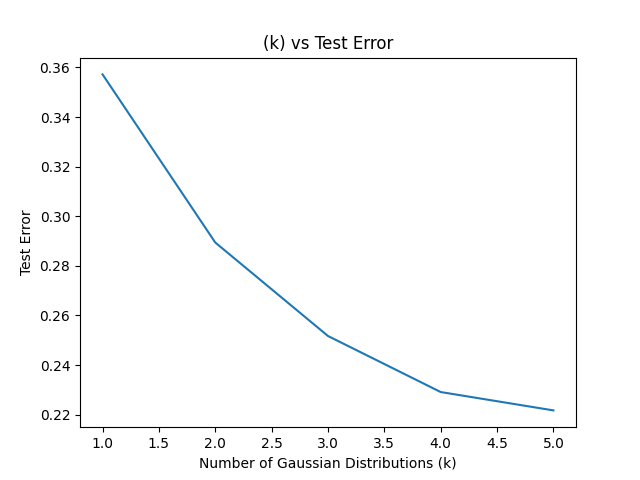
\includegraphics[width=.9\linewidth]{q3b.png}
\end{center}
With our base model we receive the following test accuracies for the perturbed test set:
\begin{center}
\begin{tabular}{||c | c |c ||} 
 \hline
 Test Accuracy on $ \epsilon = 0.1$ & Test Accuracy on $ \epsilon = 0.2$ & Test Accuracy on $ \epsilon = 0.5$ \\ [0.5ex] 
 \hline
 $76.82\%$ & $42.63\%$ & $33.88\%$ \\ 
 \hline
\end{tabular}
\end{center}
\end{titlepage}
\end{document}